\documentclass[12pt,a4paper]{report}

% ---------- Packages ----------
\usepackage[T1]{fontenc}
\usepackage[utf8]{inputenc}
\usepackage{mathptmx}
\usepackage[a4paper,left=2.5cm,right=2.5cm,top=2.5cm,bottom=2.5cm]{geometry}
\usepackage{graphicx}
\usepackage[table]{xcolor}
\usepackage{array,tabularx,longtable,booktabs}
\usepackage{enumitem}
\usepackage{caption}
\usepackage{fancyhdr}
\usepackage{titlesec}
\usepackage{tikz}
\usetikzlibrary{arrows.meta,positioning,calc,fit,backgrounds}
\usepackage[hidelinks]{hyperref}
\usepackage{setspace}
\usepackage{float}

% ---------- Colours ----------
\definecolor{headteal}{HTML}{1B4A4A}
\definecolor{tablehead}{HTML}{153F3F}
\definecolor{rowtint}{HTML}{F1F6F5}
\definecolor{boxfill}{HTML}{E6F2EF}
\definecolor{boxline}{HTML}{3D8C80}
\definecolor{sand}{HTML}{F6E7CF}
\definecolor{sandline}{HTML}{D9A766}
\definecolor{gantt}{HTML}{2E8B7E}

% ---------- Layout ----------
\setstretch{1.15}
\setlength{\parindent}{0pt}
\setlength{\parskip}{6pt}
\pagestyle{fancy}
\fancyhf{}
\fancyhead[L]{\small AI Powered Legal Advisor and Analyzer}
\fancyfoot[C]{\thepage}
\renewcommand{\headrulewidth}{0pt}
\fancypagestyle{plain}{\fancyhf{}\fancyhead[L]{\small AI Powered Legal Advisor and Analyzer}\fancyfoot[C]{\thepage}\renewcommand{\headrulewidth}{0pt}}

\titleformat{\chapter}[hang]{\normalfont\LARGE\bfseries\color{headteal}}{\thechapter}{0.6em}{}
\titlespacing*{\chapter}{0pt}{0pt}{12pt}
\titleformat{\section}{\normalfont\Large\bfseries\color{headteal}}{\thesection}{0.5em}{}
\titleformat{\subsection}{\normalfont\large\bfseries}{\thesubsection}{0.5em}{}

\renewcommand{\contentsname}{Table of Contents}
\renewcommand{\listfigurename}{List of Figures}
\renewcommand{\listtablename}{List of Tables}
\titleformat{name=\chapter,numberless}[block]{\normalfont\fontsize{22}{26}\selectfont\bfseries\filcenter}{}{0pt}{}
\titlespacing*{name=\chapter,numberless}{0pt}{0pt}{14pt}
\setcounter{tocdepth}{2}
\renewcommand{\thefigure}{\arabic{figure}}
\renewcommand{\thetable}{\arabic{table}}
\captionsetup{font={small,it},labelfont={small,it},labelsep=colon}
\captionsetup[table]{position=top,skip=4pt}

\setlist[itemize]{label=\textbullet,leftmargin=1.5em,itemsep=2pt,topsep=2pt}
\setlist[enumerate]{leftmargin=1.8em,itemsep=2pt,topsep=2pt}

% Table helpers
\newcolumntype{L}[1]{>{\raggedright\arraybackslash}p{#1}}
\newcommand{\thd}[1]{\textcolor{white}{\textbf{#1}}}
\newcommand{\headrow}{\rowcolor{tablehead}}
\renewcommand{\arraystretch}{1.3}

\usepackage{pdflscape}
\usepackage{needspace}
\setlength{\emergencystretch}{3em}
\newcommand{\fr}[4]{#1 & #2 & #3 & #4 \\ \hline}
\newcommand{\frhead}{\hline\headrow \thd{ID} & \thd{Requirement} & \thd{Actor} & \thd{Priority} \\ \hline}
\newcommand{\screen}[3]{%
  \begin{figure}[H]\centering
  \fbox{\includegraphics[width=0.94\textwidth]{figures/screens/#1}}
  \caption{#2}\label{#3}\end{figure}}

\begin{document}

% ================= TITLE PAGE =================
\begin{titlepage}
\centering
\vspace*{1.2cm}
{\fontsize{24}{30}\selectfont\bfseries AI Powered Legal Advisor and Analyzer\par}
\vspace{0.8cm}

\includegraphics[width=4.2cm]{figures/cust_logo.png}\par
\vspace{0.8cm}
{\Large\bfseries Requirements and System Design\par}
\vspace{0.1cm}
{\large Requirements, Domain Model, Class Diagram, ERD and UI/UX Prototypes\par}
\vspace{0.6cm}
{\large\bfseries Team Members\par}
\vspace{0.1cm}
{\large Muhammad Nabeel (BCS233115)\par Ashir Qureshi (BCS233084)\par Muhammad Sharjeel (BCS233113)\par}
\vspace{0.5cm}
{\large\bfseries Supervised By\par}
\vspace{0.1cm}
{\large Ms. Khadija Iftikhar\par}
\vspace{0.5cm}
{\large Fall 2026\par}
\vspace{0.2cm}
{\large Bachelor of Science in Computer Science\par}
{\large\bfseries Department of Computer Science\par}
{\large Capital University of Science \& Technology, Islamabad\par}
\vfill
\end{titlepage}
\setcounter{page}{2}

\tableofcontents
\clearpage
\listoffigures
\vspace{1.5em}
{\let\clearpage\relax\let\cleardoublepage\relax\listoftables}
\clearpage

% ================= CHAPTER 2 =================
\setcounter{chapter}{2}
\setcounter{section}{0}
\phantomsection
\addcontentsline{toc}{chapter}{Chapter 2 --- Requirements and System Design}
{\noindent\raggedright\normalfont\fontsize{22}{27}\selectfont\bfseries Chapter 2 --- Requirements and\\System Design\par}
\vspace{12pt}

This chapter turns the proposal (Chapter 1) into a concrete specification. Section~\ref{sec:fr} lists what the system must do, Section~\ref{sec:nfr} lists the qualities it must have, and the remaining sections describe the design: the domain model, the class diagram, the entity relationship diagram and the UI/UX prototypes. Throughout, we use one running example: \emph{Ali}, a tenant in Lahore whose landlord has told him to leave within seven days.

Priorities follow the MoSCoW idea in a simplified form: \textbf{High} means the feature is required for the FYP demo, \textbf{Medium} means it is planned and expected, and \textbf{Low} means it is added if time allows.

% ---------------------------------------------------------------
\section{Functional Requirements}\label{sec:fr}

\subsection{User Management and Authentication}
\begin{longtable}{|p{1.4cm}|L{9.0cm}|L{2.0cm}|L{1.6cm}|}
\caption{Functional requirements: user management and authentication}\label{tab:fr-auth}\\
\frhead\endfirsthead \frhead\endhead
\fr{FR-01}{The system shall allow a citizen to register with name, email, phone number and password.}{Citizen}{High}
\fr{FR-02}{The system shall allow a lawyer to register and submit bar licence details, specialization, city, fee range, experience and languages for verification.}{Lawyer}{High}
\fr{FR-03}{The system shall allow all users to sign in and sign out using email and password.}{All}{High}
\fr{FR-04}{The system shall restrict every page and API to the user's role (citizen, lawyer or administrator).}{System}{High}
\fr{FR-05}{The system shall allow users to update their profile and reset a forgotten password by email.}{All}{Medium}
\end{longtable}

\subsection{Case Management and Fact Clarification}
\begin{longtable}{|p{1.4cm}|L{9.0cm}|L{2.0cm}|L{1.6cm}|}
\caption{Functional requirements: case management and fact clarification}\label{tab:fr-case}\\
\frhead\endfirsthead \frhead\endhead
\fr{FR-06}{The system shall allow a citizen to create a case by entering a title and a description of the problem in their own words.}{Citizen}{High}
\fr{FR-07}{The system shall detect the legal area (property or family) and the likely topic of a new case, and allow the citizen to correct it.}{System}{High}
\fr{FR-08}{The system shall identify facts that are missing for the detected topic and ask the citizen only the follow-up questions needed to fill them.}{System}{High}
\fr{FR-09}{The system shall store every follow-up question and answer as part of the case.}{System}{High}
\fr{FR-10}{The system shall show the citizen a list of their cases with title, legal area, status and last update.}{Citizen}{High}
\fr{FR-11}{The system shall allow a citizen to close or delete their own case.}{Citizen}{Medium}
\end{longtable}

\subsection{Document and Evidence Processing}
\begin{longtable}{|p{1.4cm}|L{9.0cm}|L{2.0cm}|L{1.6cm}|}
\caption{Functional requirements: document and evidence processing}\label{tab:fr-doc}\\
\frhead\endfirsthead \frhead\endhead
\fr{FR-12}{The system shall allow a citizen to upload PDF, JPG and PNG files to a case.}{Citizen}{High}
\fr{FR-13}{The system shall extract text from digital PDFs using PyMuPDF.}{System}{High}
\fr{FR-14}{The system shall extract text from scanned files and photos using OCR.}{System}{High}
\fr{FR-15}{The system shall identify key clauses (for example rent, term, notice period) in an uploaded agreement and show them to the citizen.}{System}{Medium}
\fr{FR-16}{The system shall generate a case-specific evidence checklist and mark an item as ready when a matching document is uploaded.}{System}{High}
\end{longtable}

\subsection{RAG Legal Guidance}
\begin{longtable}{|p{1.4cm}|L{9.0cm}|L{2.0cm}|L{1.6cm}|}
\caption{Functional requirements: RAG legal guidance}\label{tab:fr-rag}\\
\frhead\endfirsthead \frhead\endhead
\fr{FR-17}{The system shall convert the clarified case into a query embedding using Sentence Transformers.}{System}{High}
\fr{FR-18}{The system shall retrieve the top-$k$ most similar law sections from the Qdrant vector database, filtered by legal area.}{System}{High}
\fr{FR-19}{The system shall send the open-source LLM a grounded prompt containing only the retrieved sections, the case facts and the instruction to answer only from those sections.}{System}{High}
\fr{FR-20}{The system shall attach a citation (act, section and quoted text) to every statement in the answer.}{System}{High}
\fr{FR-21}{The system shall check that every citation in a generated answer refers to a retrieved section before the answer is shown; answers that fail the check shall not be shown.}{System}{High}
\fr{FR-22}{If no relevant verified source is found, the system shall tell the citizen so and suggest consulting a verified lawyer instead of guessing.}{System}{High}
\fr{FR-23}{The system shall present the answer in plain language together with a list of sources and a disclaimer that it does not replace a lawyer.}{Citizen}{High}
\fr{FR-24}{The system shall allow the citizen to ask a further question within the same case, using the stored case facts.}{Citizen}{Medium}
\end{longtable}

\subsection{Lawyer Directory, Case Sharing and Tracking}
\begin{longtable}{|p{1.4cm}|L{9.0cm}|L{2.0cm}|L{1.6cm}|}
\caption{Functional requirements: lawyer directory, sharing and tracking}\label{tab:fr-lawyer}\\
\frhead\endfirsthead \frhead\endhead
\fr{FR-25}{The system shall list only administrator-verified lawyers in the directory.}{System}{High}
\fr{FR-26}{The system shall allow a citizen to filter lawyers by specialization, city, fee range, experience, language and rating.}{Citizen}{High}
\fr{FR-27}{The system shall show a lawyer profile with verification badge, specialization, fee range, experience, languages and reviews.}{Citizen}{High}
\fr{FR-28}{The system shall share a case with a lawyer only after the citizen gives explicit consent, and shall show what will be shared.}{Citizen}{High}
\fr{FR-29}{The system shall allow a citizen to stop sharing a case at any time.}{Citizen}{Medium}
\fr{FR-30}{The system shall allow a lawyer to accept or decline a shared case.}{Lawyer}{High}
\fr{FR-31}{The system shall allow a lawyer to post status updates and notes on an accepted case.}{Lawyer}{High}
\fr{FR-32}{The system shall show the citizen a timeline of all status changes for a case until it is resolved.}{Citizen}{High}
\fr{FR-33}{The system shall notify the citizen in the application when the status of their case changes.}{System}{Medium}
\fr{FR-34}{The system shall allow a citizen to rate and review a lawyer after a shared case is resolved.}{Citizen}{Low}
\end{longtable}

\subsection{Administration and Knowledge Base}
\begin{longtable}{|p{1.4cm}|L{9.0cm}|L{2.0cm}|L{1.6cm}|}
\caption{Functional requirements: administration and knowledge base}\label{tab:fr-admin}\\
\frhead\endfirsthead \frhead\endhead
\fr{FR-35}{The system shall allow an administrator to approve or reject a lawyer's verification request after reviewing the submitted licence.}{Admin}{High}
\fr{FR-36}{The system shall allow an administrator to add a verified legal source (act, ordinance or rules) to the knowledge base.}{Admin}{High}
\fr{FR-37}{The system shall split each new legal source into section-wise chunks with metadata, create embeddings and store them in Qdrant.}{System}{High}
\fr{FR-38}{The system shall allow an administrator to deactivate users and remove inappropriate content.}{Admin}{Medium}
\fr{FR-39}{The system shall show the administrator a dashboard with counts of users, verified lawyers, open cases and indexed law sections.}{Admin}{Medium}
\end{longtable}

% ---------------------------------------------------------------
\section{Non-Functional Requirements}\label{sec:nfr}
The targets below are design goals. They will be measured during testing and evaluation (work packages 16--18) and adjusted if the deployment hardware requires it.

\begin{longtable}{|p{1.5cm}|L{2.6cm}|L{10.1cm}|}
\caption{Non-functional requirements}\label{tab:nfr}\\
\hline\headrow \thd{ID} & \thd{Category} & \thd{Requirement and target} \\ \hline\endfirsthead
\hline\headrow \thd{ID} & \thd{Category} & \thd{Requirement and target} \\ \hline\endhead
NFR-01 & Performance & Pages other than guidance generation shall load within 2 seconds for 95\% of requests. \\ \hline
NFR-02 & Performance & Law-section retrieval from Qdrant shall complete within 1 second; a full guidance answer shall be produced within 30 seconds for 90\% of requests on the deployment server, with a progress indicator shown meanwhile. \\ \hline
NFR-03 & Accuracy and grounding & Every statement in a guidance answer shall be backed by a citation to a retrieved, verified source. The RAG system shall score higher than the standard LLM baseline on the defined quality measures. \\ \hline
NFR-04 & Security & Passwords shall be stored only as salted hashes (bcrypt or Argon2). All traffic shall use HTTPS. APIs shall use token-based authentication with role checks on every request. \\ \hline
NFR-05 & Security & Uploaded documents and case text shall be treated as data only and never as instructions to the LLM, to protect against prompt injection. \\ \hline
NFR-06 & Privacy & A case shall be visible only to its citizen, to lawyers the citizen has consented to share it with, and to administrators for moderation. Citizens shall be able to delete their case data. \\ \hline
NFR-07 & Usability & A first-time citizen shall be able to create a case and read guidance without help. The system shall reach a System Usability Scale (SUS) score of at least 68. \\ \hline
NFR-08 & Usability & Guidance shall be written in plain language that avoids unexplained legal terms. \\ \hline
NFR-09 & Accessibility & The web portals shall be usable on desktop and mobile screens (responsive design) and meet basic WCAG 2.1 AA contrast. \\ \hline
NFR-10 & Reliability & If the LLM or OCR service fails, the system shall show a clear error and keep the case and uploaded files without loss. \\ \hline
NFR-11 & Availability & The deployed system shall target 99\% uptime during the evaluation period. \\ \hline
NFR-12 & Scalability & The backend, MongoDB and Qdrant shall be separate components so that each can be scaled or replaced independently. \\ \hline
NFR-13 & Maintainability & New legal areas shall be addable by ingesting new verified sources, without code changes to the RAG pipeline. Code shall be version-controlled in Git with documented APIs. \\ \hline
NFR-14 & Portability & Development shall be possible on Windows, Linux and macOS; deployment shall run on a Linux server. \\ \hline
NFR-15 & Legal and ethical & Every guidance page shall state that the platform does not replace a qualified lawyer. Only administrator-verified lawyers and sources shall be shown. \\ \hline
\end{longtable}

% ---------------------------------------------------------------
\section{Domain Model}\label{sec:domain}
The domain model (Figure~\ref{fig:domain}) shows the main concepts of the problem and how they relate, without any software detail. A \emph{Citizen} opens a \emph{Case}. The case is clarified by \emph{Follow-up Questions}, may have \emph{Uploaded Documents} containing \emph{Clauses}, and receives \emph{Legal Guidance}. Each piece of guidance is supported by \emph{Citations} that quote a \emph{Law Section} of a verified \emph{Legal Source}. A case may have an \emph{Evidence Checklist}, and through a \emph{Case Share}, given with the citizen's consent, it can be handed to a \emph{Lawyer}. \emph{Status Updates} record the case history, and the \emph{Administrator} verifies both lawyers and legal sources.

\begin{landscape}
\begin{figure}[p]
\centering
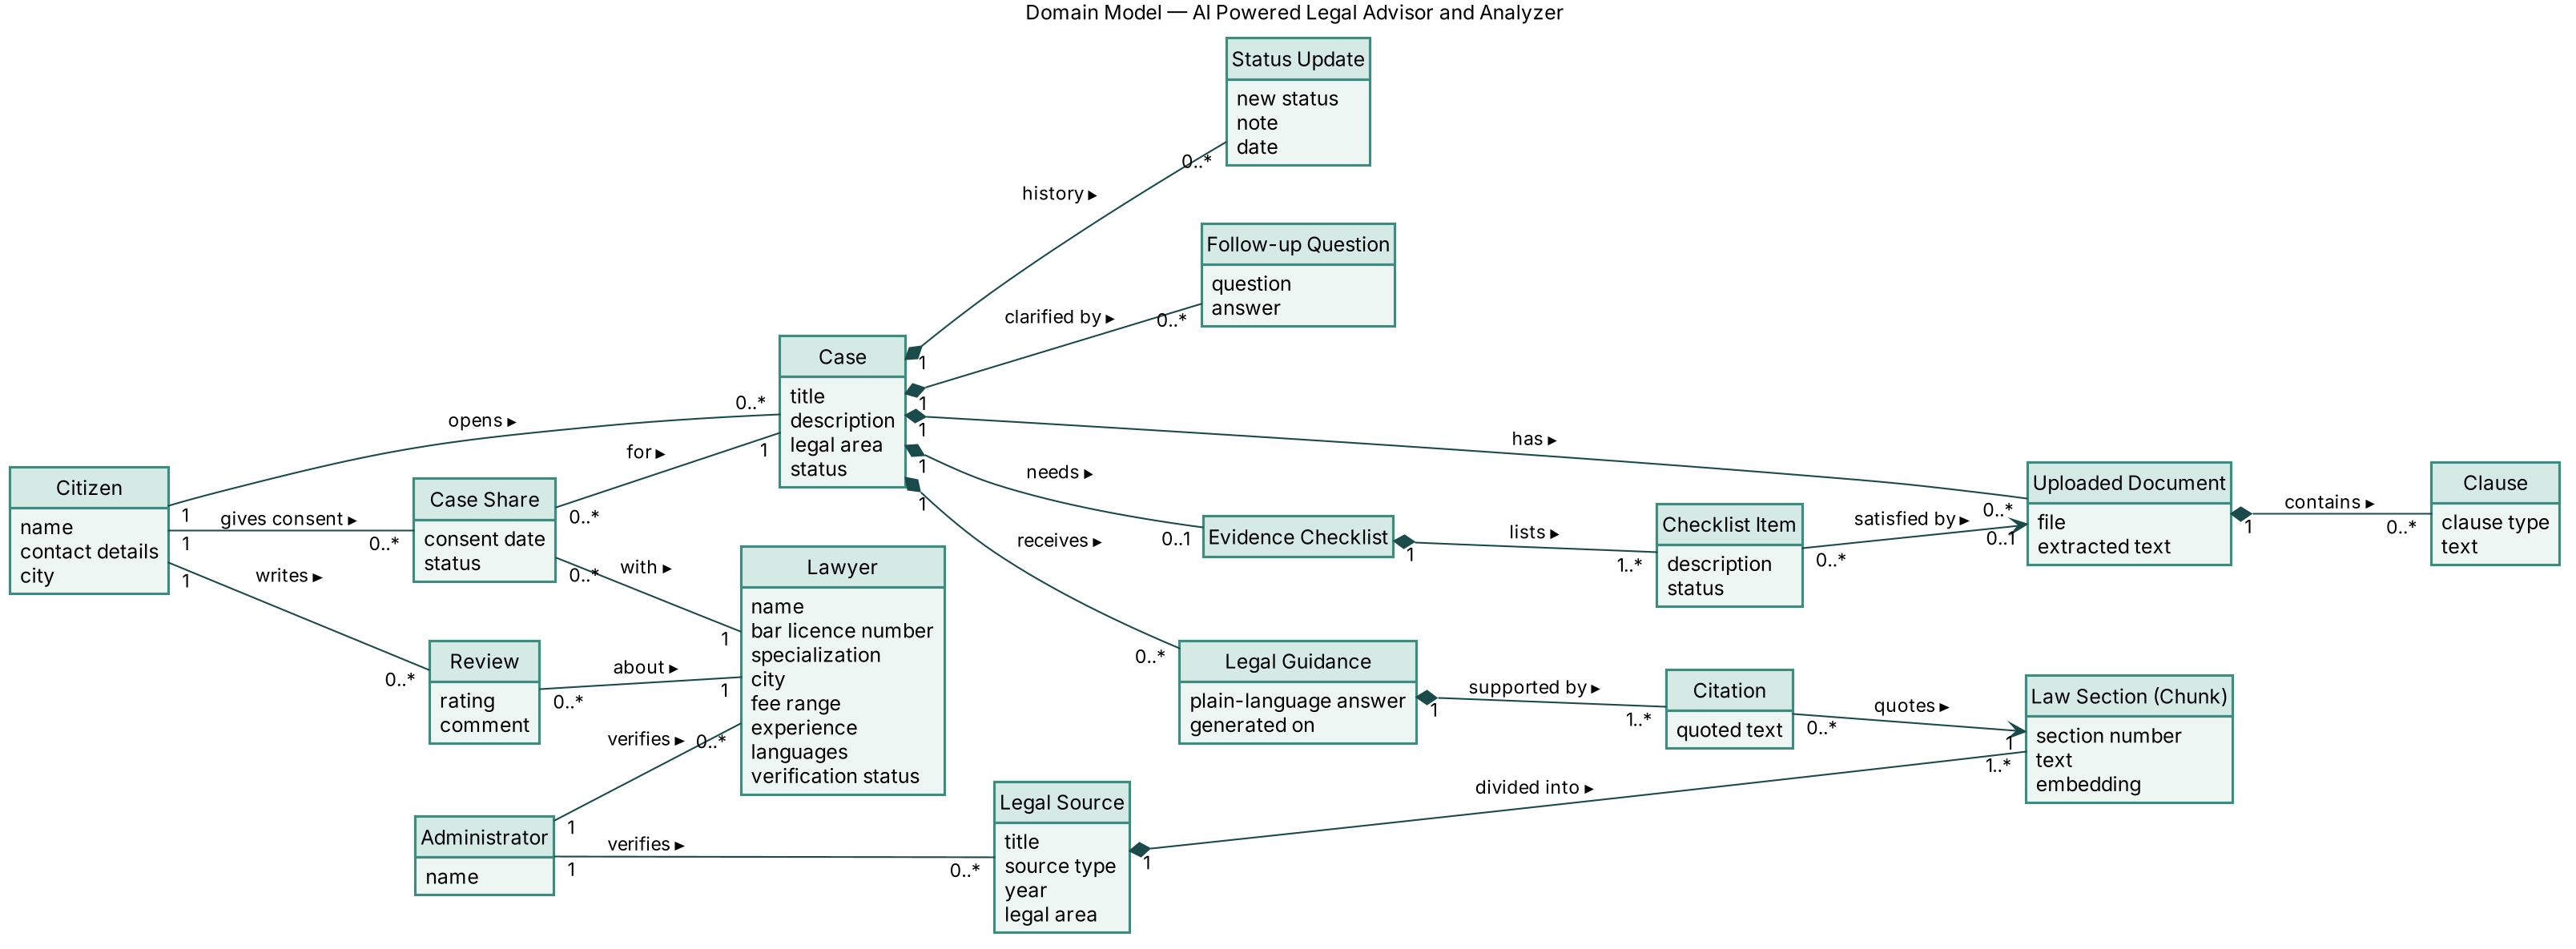
\includegraphics[width=24.5cm,height=14.6cm,keepaspectratio]{figures/domain_model.png}
\caption{Domain model}\label{fig:domain}
\end{figure}
\end{landscape}

% ---------------------------------------------------------------
\section{Class Diagram}\label{sec:class}
The class diagram is split into two parts so that it stays readable.

\textbf{Part A (Figure~\ref{fig:class-a})} shows the domain classes that the system stores. \texttt{User} is an abstract class with three subclasses: \texttt{Citizen}, \texttt{Lawyer} and \texttt{Administrator}. A lawyer owns exactly one \texttt{LawyerProfile}, which holds the verification status and the data used by the directory filters. \texttt{Case} is the centre of the model: it is composed of follow-up questions, documents, guidance, a checklist, shares and status updates. Enumerations fix the allowed values of case status, legal area, verification status and share status.

\textbf{Part B (Figure~\ref{fig:class-b})} shows the application services and how the RAG pipeline is built. \texttt{RAGService} coordinates the \texttt{EmbeddingService} (Sentence Transformers), the \texttt{Retriever} (backed by \texttt{QdrantStore}), the \texttt{LLMClient} (open-source LLM), the \texttt{CitationChecker} and the \texttt{ChecklistGenerator}. The LLM client has no link to any data store: it only ever receives the law sections that \texttt{RAGService} retrieved. \texttt{KnowledgeBaseBuilder} is used by the administrator to ingest new verified sources.

\begin{figure}[p]
\centering
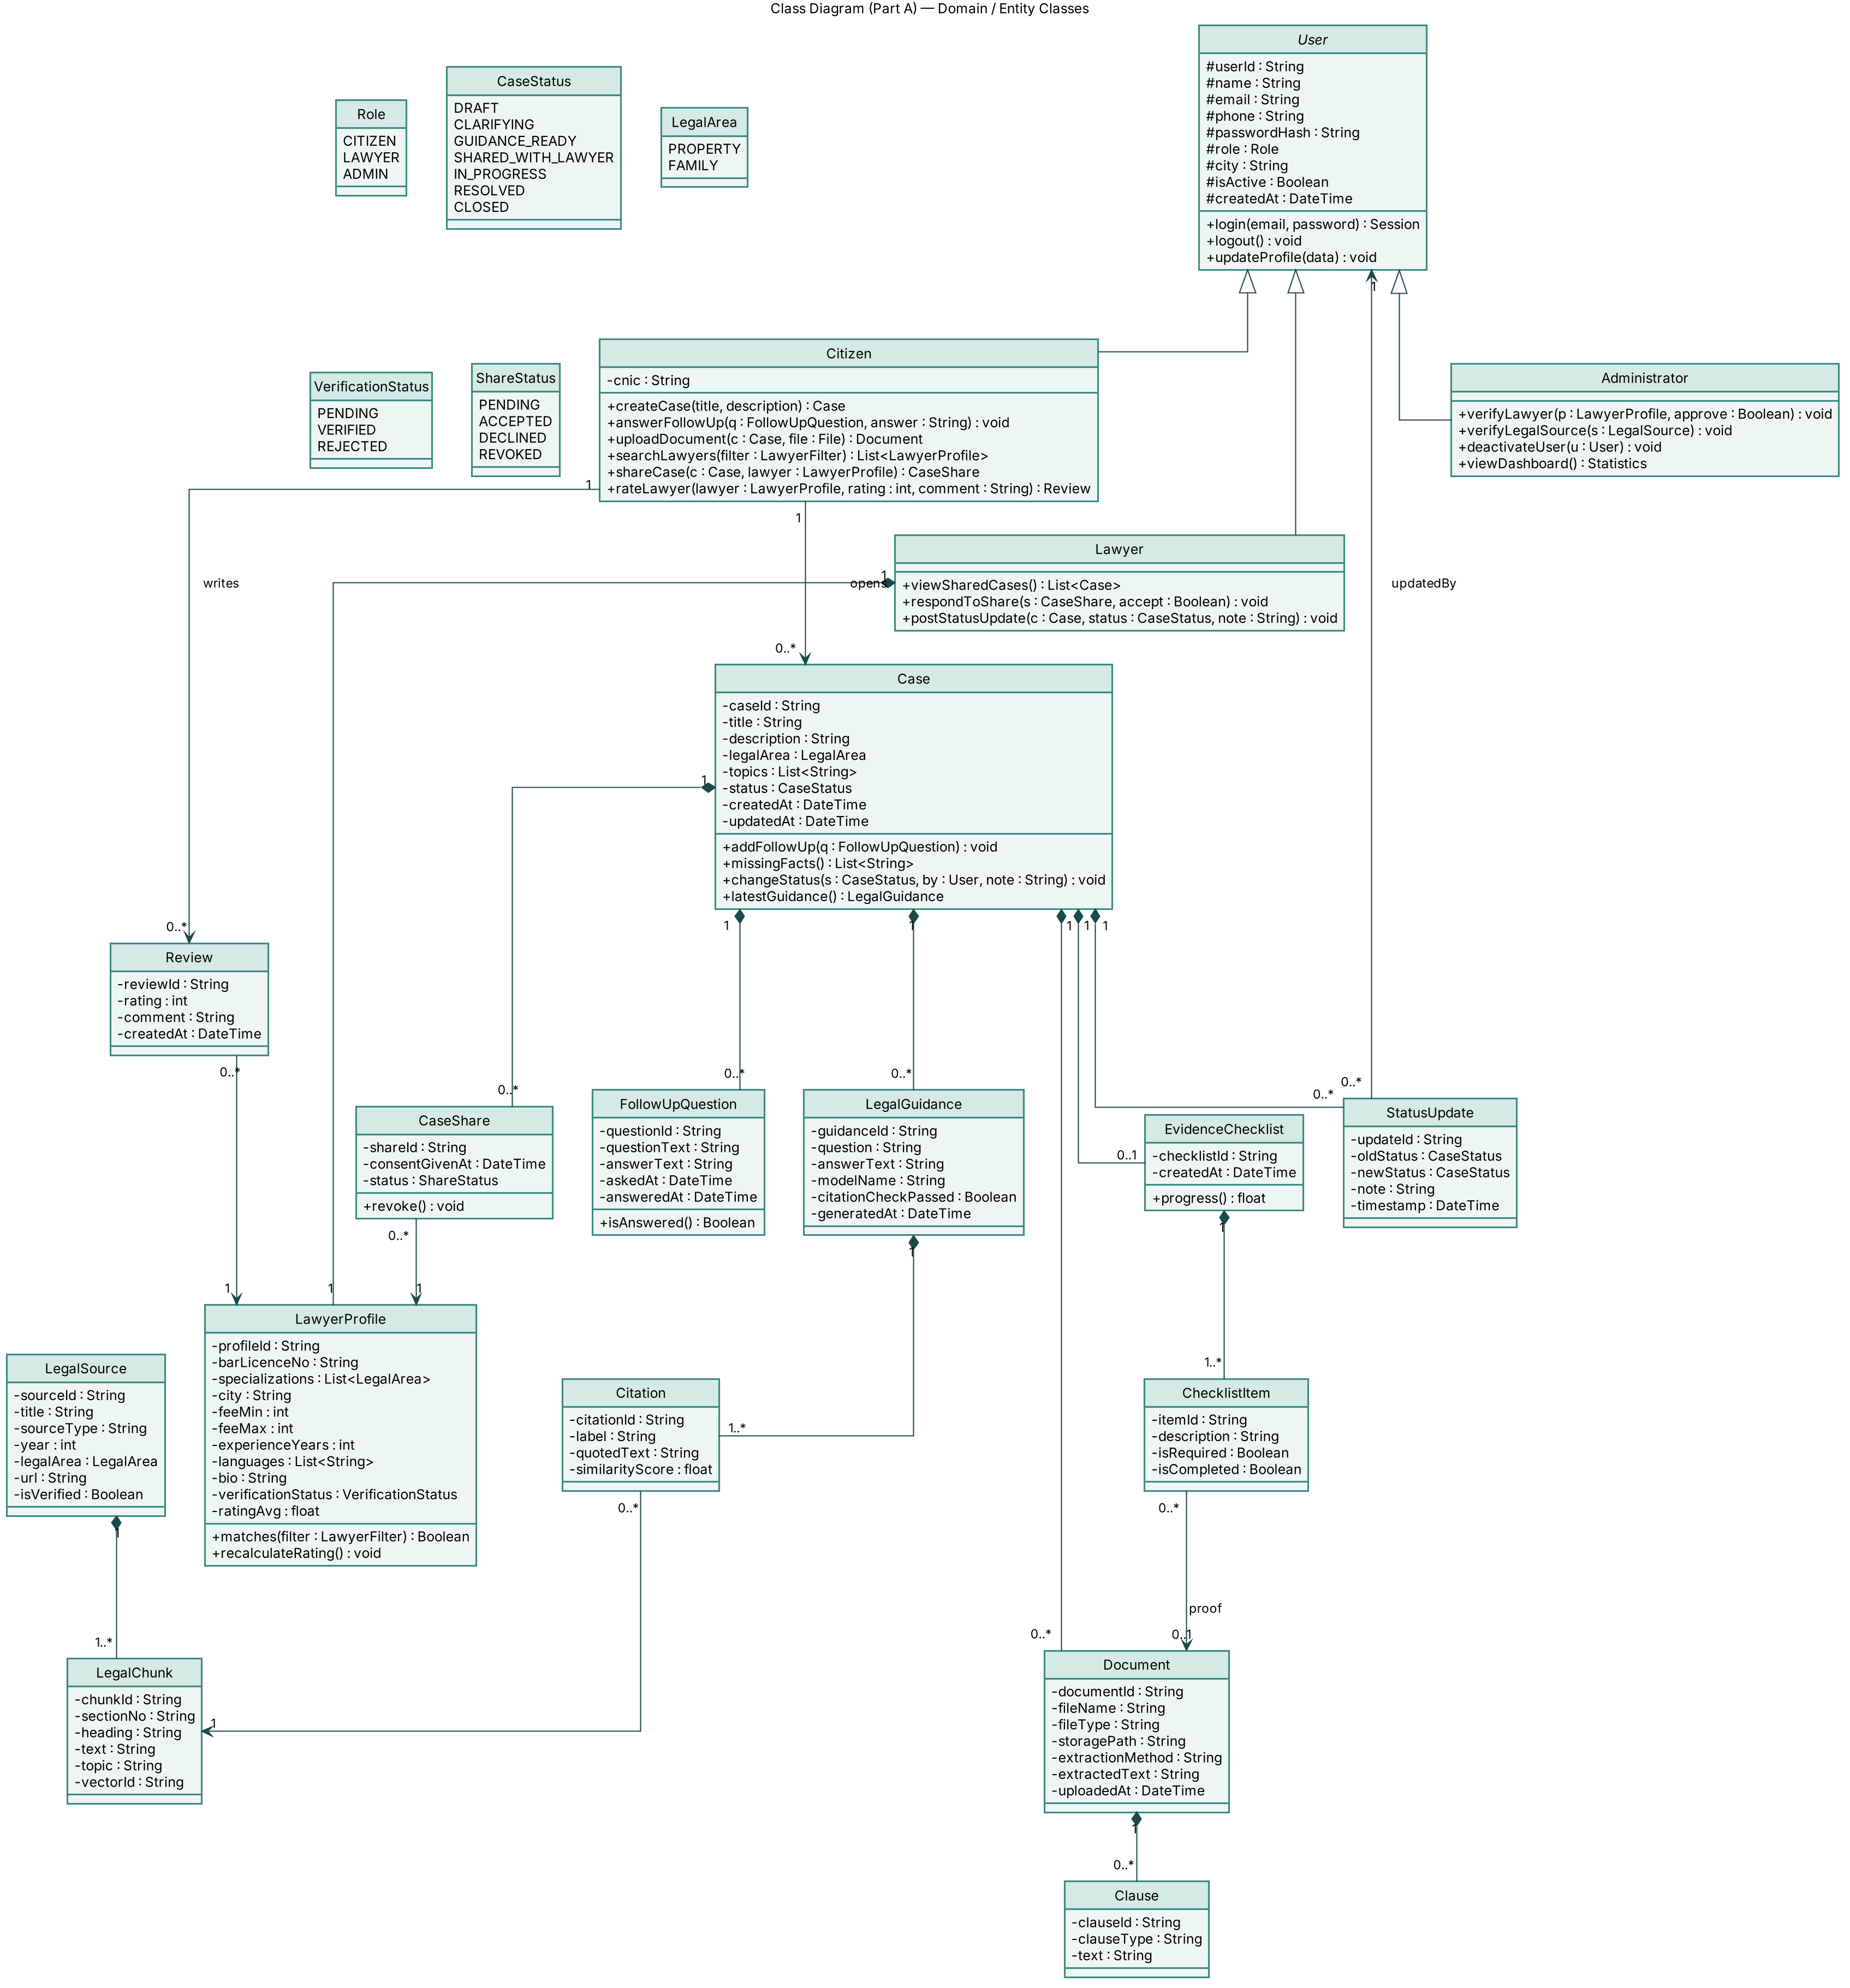
\includegraphics[width=\textwidth,height=0.86\textheight,keepaspectratio]{figures/class_entities.png}
\caption{Class diagram, Part A: domain and entity classes}\label{fig:class-a}
\end{figure}

\begin{landscape}
\begin{figure}[p]
\centering
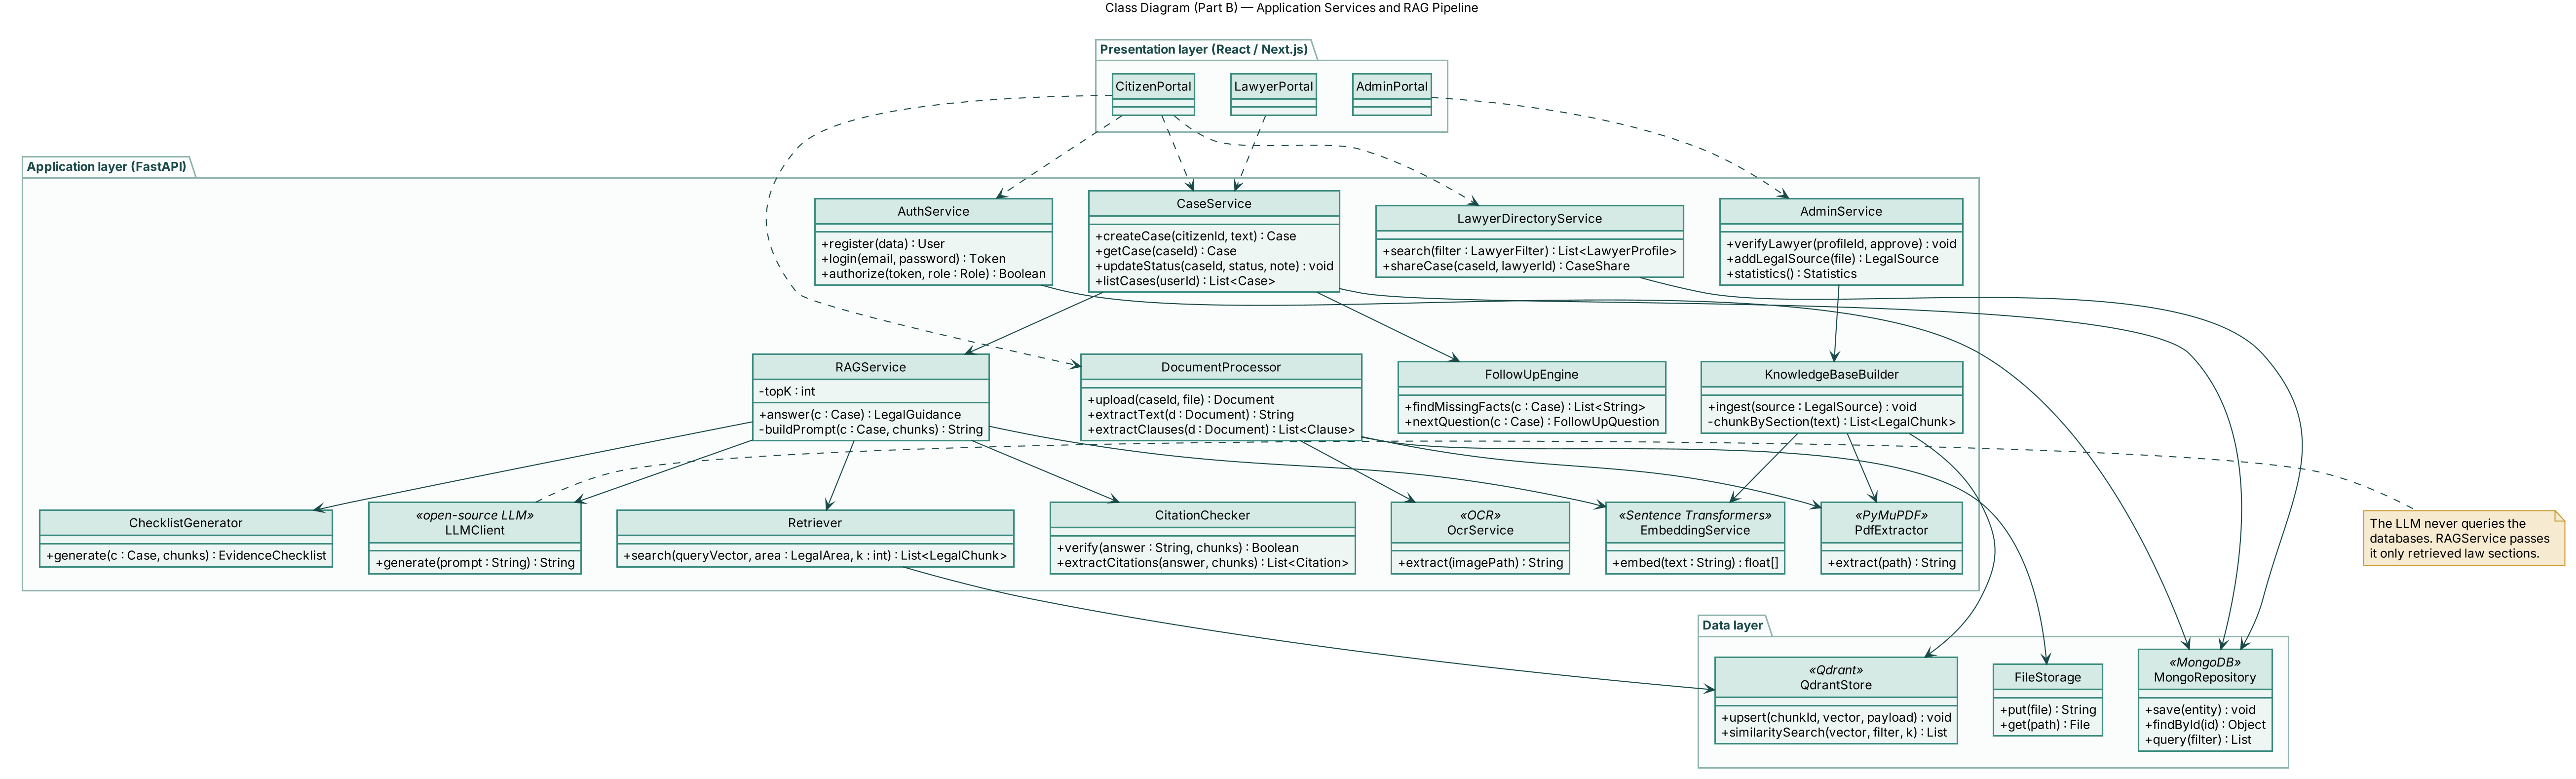
\includegraphics[width=24.5cm,height=14.6cm,keepaspectratio]{figures/class_services.png}
\caption{Class diagram, Part B: application services and RAG pipeline}\label{fig:class-b}
\end{figure}
\end{landscape}

% ---------------------------------------------------------------
\section{Entity Relationship Diagram}\label{sec:erd}
Figure~\ref{fig:erd} gives the logical ERD using crow's-foot notation. Each entity becomes a MongoDB collection; primary keys are MongoDB \texttt{ObjectId}s and relationships are stored as reference fields (FK). The \texttt{legal\_vectors} entity (highlighted) lives in Qdrant rather than MongoDB: each Qdrant point holds the embedding of one law section and carries the section's \texttt{chunk\_id} in its payload, so a retrieval result can always be traced back to its source act and section.

\begin{table}[H]
\centering
\caption{Main relationships in the ERD}\label{tab:erd-rel}
\begin{tabular}{|L{4.6cm}|L{2.4cm}|L{7.4cm}|}
\hline\headrow \thd{Relationship} & \thd{Cardinality} & \thd{Meaning} \\ \hline
users -- cases & 1 : 0..* & A citizen can open many cases. \\ \hline
users -- lawyer\_profiles & 1 : 0..1 & Only users with the lawyer role have a profile. \\ \hline
cases -- legal\_guidance & 1 : 0..* & A case can receive several answers over time. \\ \hline
legal\_guidance -- citations & 1 : 1..* & Every answer must have at least one citation. \\ \hline
legal\_chunks -- citations & 1 : 0..* & A law section can be cited by many answers. \\ \hline
legal\_sources -- legal\_chunks & 1 : 1..* & Each source is split into sections. \\ \hline
legal\_chunks -- legal\_vectors & 1 : 1 & Each section has exactly one embedding in Qdrant. \\ \hline
cases -- case\_shares -- lawyer\_profiles & M : N & A case can be shared with several lawyers, and a lawyer receives many cases; \texttt{case\_shares} resolves this with the consent date and status. \\ \hline
cases -- evidence\_checklists & 1 : 0..1 & A case has at most one checklist. \\ \hline
\end{tabular}
\end{table}

\begin{landscape}
\begin{figure}[p]
\centering
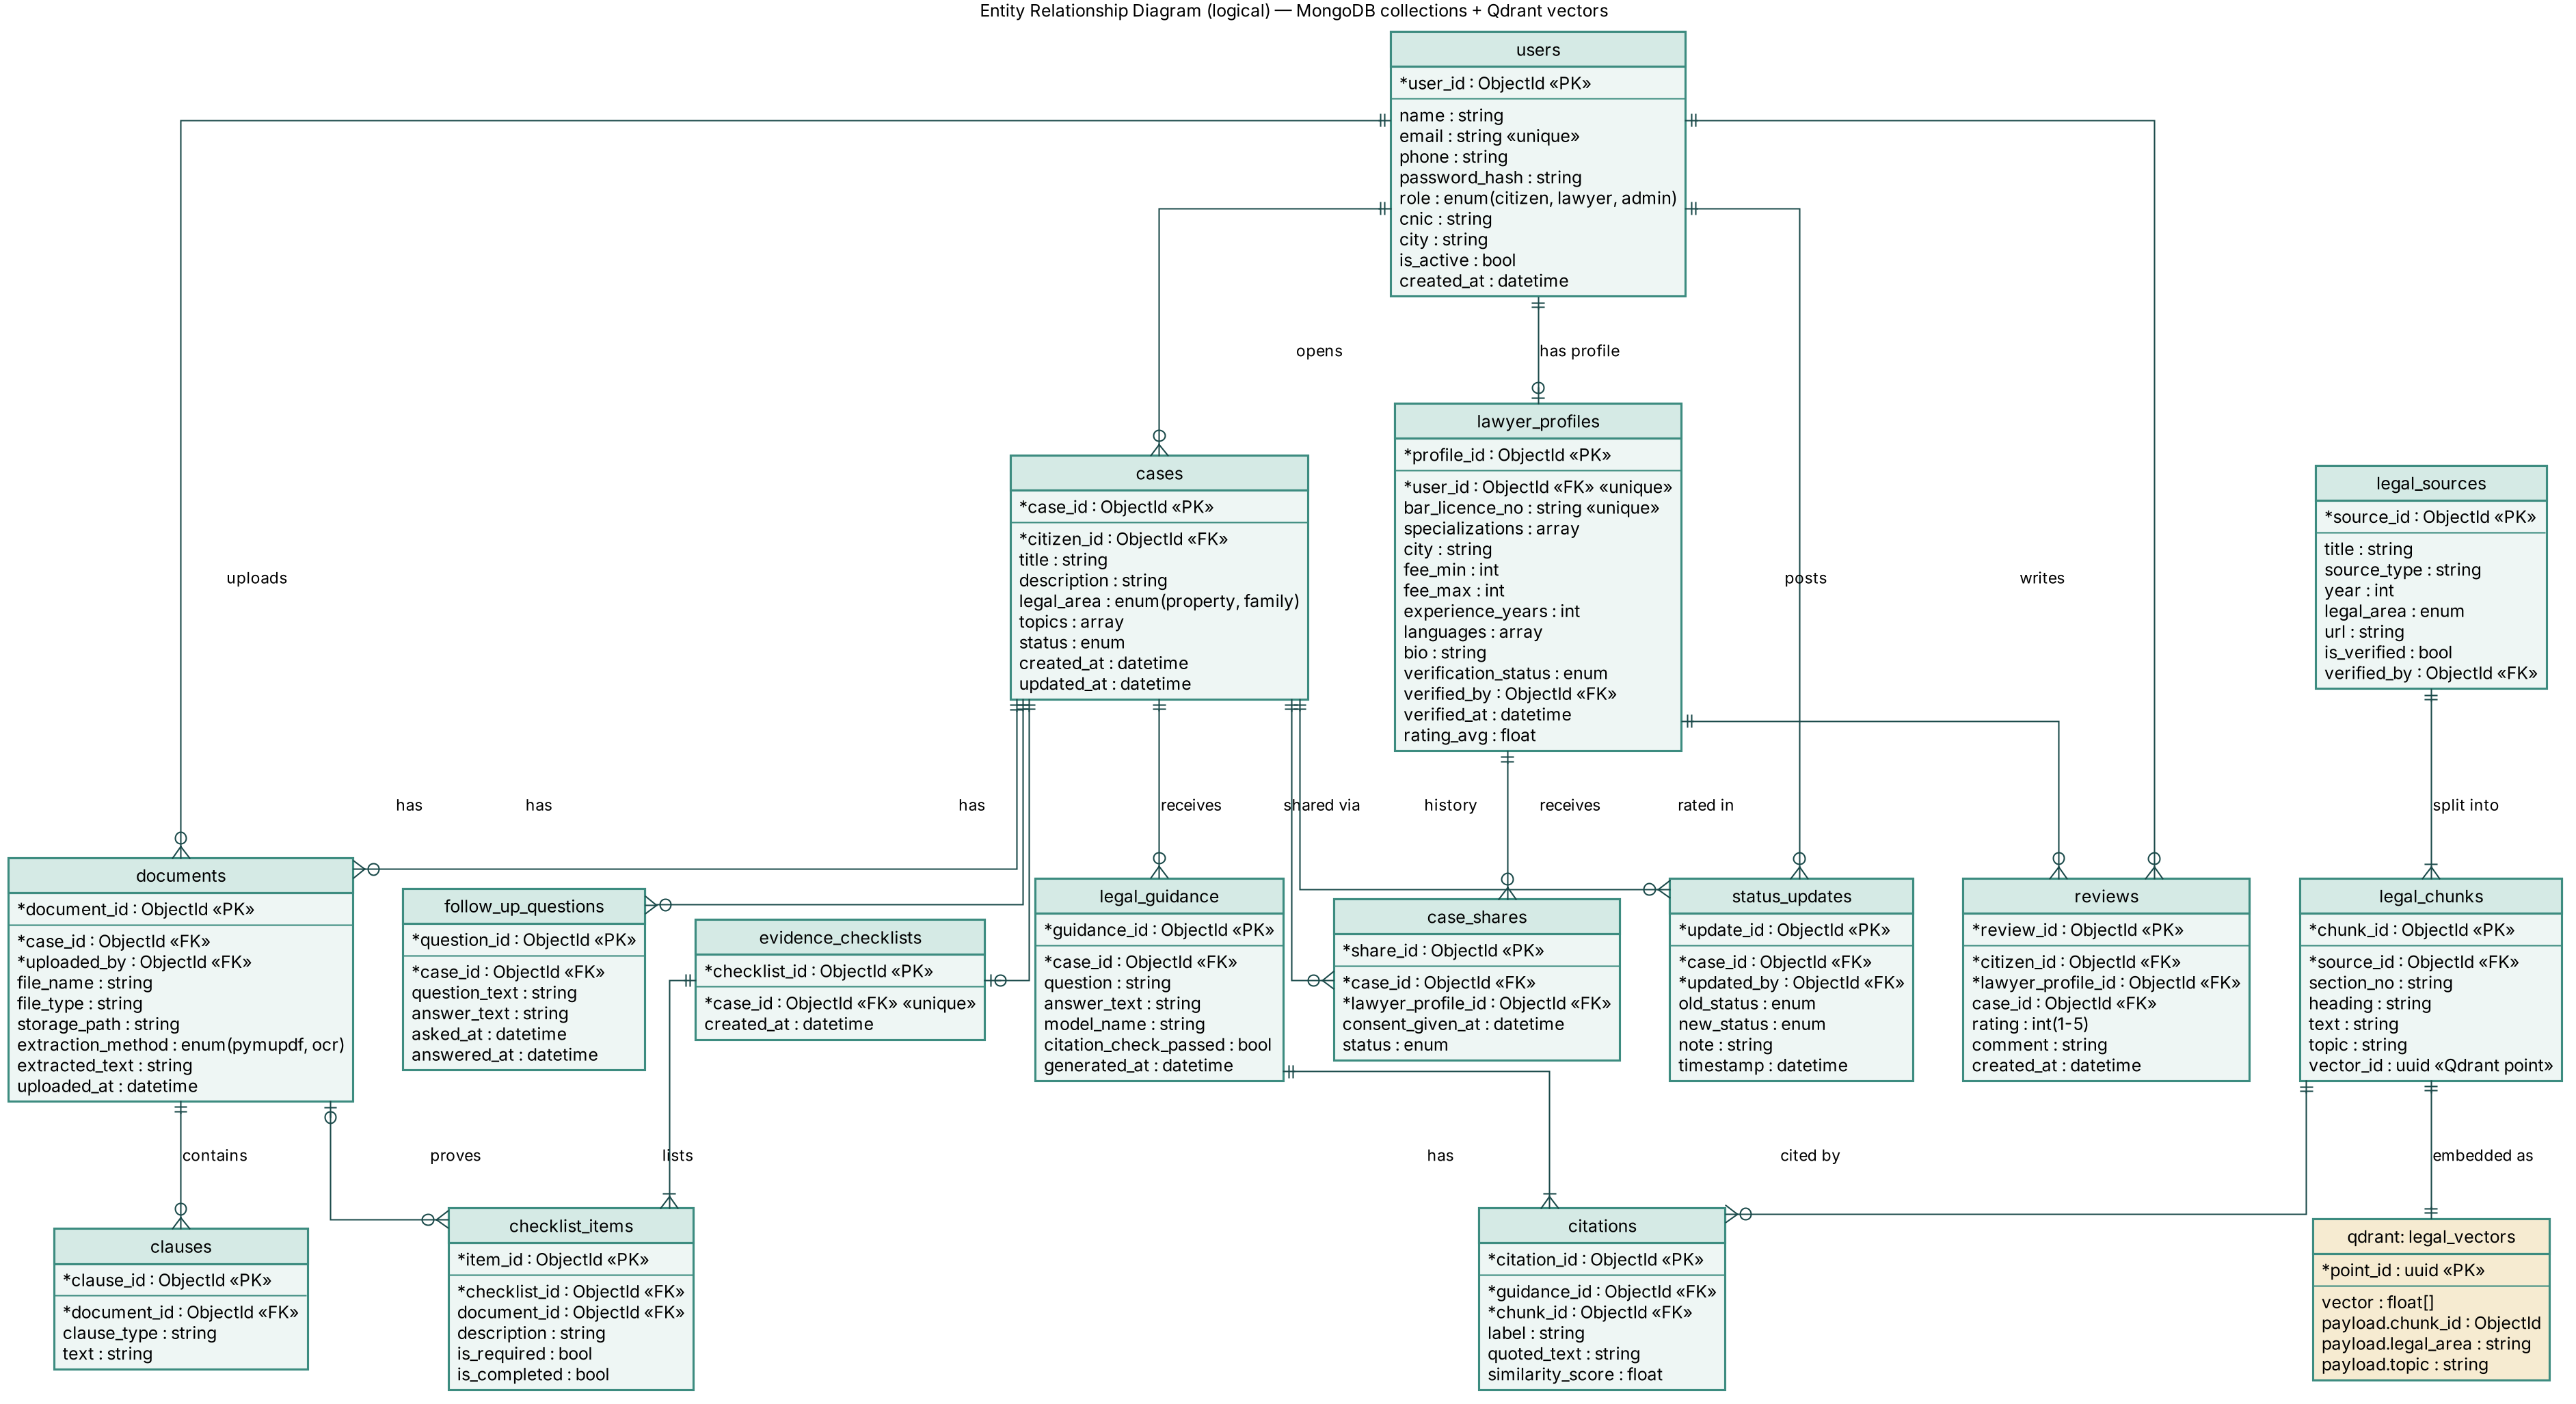
\includegraphics[width=24.5cm,height=14.6cm,keepaspectratio]{figures/erd.png}
\caption{Entity relationship diagram (MongoDB collections and Qdrant vectors)}\label{fig:erd}
\end{figure}
\end{landscape}

% ---------------------------------------------------------------
\section{UI/UX Prototypes}\label{sec:ui}
The prototypes below are high-fidelity mock-ups of the three portals. They follow the case journey of our running example, Ali. A clickable HTML version of the same screens accompanies this document. Names, figures and legal text in the screens are sample data.

\textbf{Design principles.}
\begin{itemize}
  \item \textbf{Plain language first.} Labels and guidance avoid legal jargon; legal terms are explained where they appear.
  \item \textbf{Proof is always visible.} Every guidance statement carries a source tag (S1, S2, \ldots) that links to the act and section.
  \item \textbf{Ask, don't assume.} The system asks short follow-up questions and shows which facts are still missing.
  \item \textbf{Consent before sharing.} The citizen sees exactly what a lawyer will receive before sharing a case, and can stop sharing at any time.
  \item \textbf{Consistent layout.} All portals use the same sidebar, colours and components, so users moving between screens are never lost.
\end{itemize}

\screen{01_login.png}{Sign in screen with role selection}{fig:ui-login}
\screen{02_dashboard.png}{Citizen dashboard: case list and status}{fig:ui-dash}
\screen{03_newcase.png}{New case: the citizen describes the problem; the legal area is detected}{fig:ui-new}
\screen{04_followup.png}{Follow-up questions: only the missing facts are asked}{fig:ui-follow}
\screen{05_guidance.png}{Legal guidance with source tags, sources table and evidence checklist}{fig:ui-guide}
\screen{06_documents.png}{Document upload: PyMuPDF and OCR extraction with key clauses}{fig:ui-docs}
\screen{07_directory.png}{Lawyer directory with filters (verified lawyers only)}{fig:ui-dir}
\screen{08_profile.png}{Lawyer profile and consent dialog before sharing a case}{fig:ui-share}
\screen{09_tracking.png}{Case tracking timeline}{fig:ui-track}
\screen{10_lawyer.png}{Lawyer portal: shared case requests and status updates}{fig:ui-lawyer}
\screen{11_admin.png}{Admin portal: lawyer verification and legal knowledge base}{fig:ui-admin}

\end{document}
